\chapter{Tourism in India} % (fold)
\label{cha:tii}

In the long panorama of India's history, wrote Nehru:

\begin{quote}
  There were men who seemed to know life and understood it, and out of their wisdom, they built a structure that gave India a cultural stability which lasted thousands of years.
\end{quote}

\noindent Mark Twain in his book, \emph{Following the Equator -- A journey around the world}, sums-up the enigma that is India and its unlimited potential in terms of its rich heritage and its teeming diversity: 

\begin{quote}
  The land of dreams and romance, of fabulous wealth and fabulous poverty, of splendour and rags, of palaces and hovels, of famine and pestilence, of genii and giants and Aladdin lamps, of tigers and elephants, the cobra and the jungle, the country of a hundred nations and a hundred tongues, of a thousand religions and two million gods, cradle of the human race, birthplace of human speech, mother of history, grandmother of legend, great grandmother of tradition, whose yesterdays bear date with the mouldering antiquities of the rest of the nations --- the one sole country under the sun that is endowed with an imperishable interest for alien prince and alien peasant, for lettered and ignorant, wise and fool, rich and poor, bond and free, the one land that all men desire to see, and having seen once, by even a glimpse, would not give that glimpse for the shows of all the rest of the globe combined.
\end{quote}

\noindent The cast and beautiful country that is India, its rich and colourful attractions deserves a substantially greater inflow than it currently does. \autoref{tab:tarr} offers a breakdown of tourists arriving in India.\footnote{Source: Department of Tourism, Mumbai.}

\begin{table}[H]
\caption{Tourist arrivals in India}
\label{tab:tarr}
\centering
  \begin{tabular}{+r^r^r^r^r^r}
  \rowstyle{\itshape}
        & 1993 & 1994 & 1995 & 1996 & 1997  \\ %& 94-93 & 95-94 & 96-95 & 97-96 \\
    Jan & 150,019 & 192,551 & 197,343 & 224,029 & 240,569 \\ % &  23.4 &  2.5 & 13.5 &  7.4 \\
    Feb & 119,680 & 172,642 & 187,614 & 219,635 & 227,458 \\ % &  15.3 &  8.7 & 17.1 &  3.6 \\
    Mar & 146,191 & 187,129 & 188,252 & 196,196 & 218,411 \\ % &  28.0 &  0.6 &  4.2 & 11.3 \\
    Apr & 118,200 & 142,501 & 146,715 & 158,785 & 154,863 \\ % &  20.6 &  3.0 &  8.2 & -2.5 \\
    May & 103,371 & 120,183 & 122,918 & 132,833 & 137,536 \\ % &  16.3 &  2.3 &  8.1 &  3.5 \\
    Jun & 118,171 & 124,908 & 128,137 & 133,154 & 143,199 \\ % &   5.7 &  2.6 &  3.9 &  7.5 \\
    Jul & 148,255 & 168,969 & 171,458 & 176,347 & 184,324 \\ % &  14.0 &  1.5 &  2.0 &  4.5 \\
    Aug & 136,917 & 159,519 & 159,892 & 167,985 &         \\ % &  16.1 &  0.2 &  5.1 & \\
    Sep & 125,693 & 133,995 & 150,261 & 160,840 &         \\ % &   6.6 & 12.1 &  7.0 & \\
    Oct & 165,048 & 170,609 & 196,682 & 204,126 &         \\ % & -34.8 & 22.8 &  2.8 & \\
    Nov & 188,877 & 156,926 & 221,524 & 240,620 &         \\ % & -16.9 & 41.2 &  8.6 & \\
    Dec & 214,408 & 219,501 & 252,887 & 273,310 &         \\ % &   2.4 & 1502 &  8.1 & \\
  Total & 1,734,830 & 1,949,433 & 2,123,683 & 2,287,860 & 1,306,360 \\
  \end{tabular}
\end{table}

\section{Effects of tourism on the economy} % (fold)
\label{sec:etoe}

India has seen a non-linear growth since its independence in 1947. Non-national visitors grew from 16,829 in 1951 to 16,25,950 in 1997. The per capita tourist expenditure rose from about Rs. 4,400 in 1976 to about Rs. 21,000 in 1996 approximately the same in both packaged and non-packaged categories. As a result, tourism is already an important segment that is making notable contributions to India's economy, see \autoref{fig:earn} for foreign exchange earnings.\footnote{Source: Annual report, 1995-6, Ministry of Tourism, New Delhi.} Infrastructure improvements to international norms has the potential to earn Rs. 60 Billion annually in the next five years.

The investment in tourism is on a modest scale and the returns are swift. The attractions of a region are its sources of tourism. Investments in accessibility (air, rail, road, and waterways, where practicable) and accommodation (budget and premium) would be key enablers.

\begin{figure}[H]
  \centering
  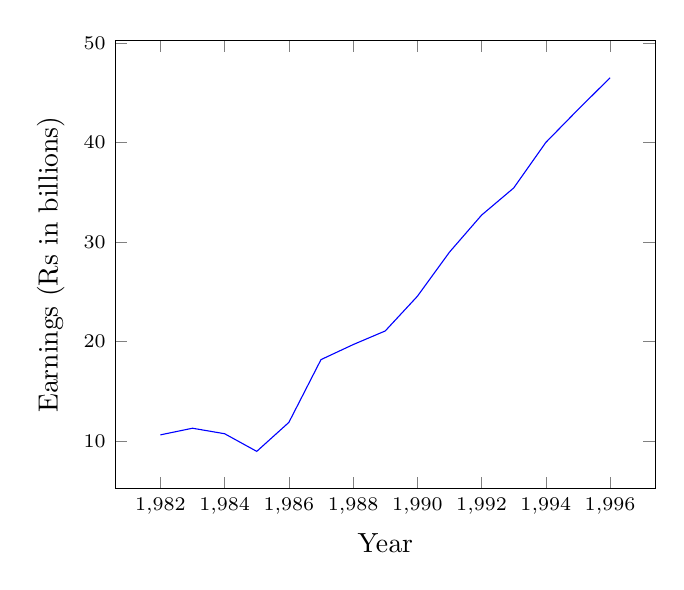
\begin{tikzpicture}
  \begin{axis}[
    no markers,
    xlabel=Year,
    xticklabel style={font=\scriptsize}, 
    ylabel=Earnings (Rs in billions),
    yticklabel style={font=\scriptsize}
    ]
    \addplot table[x=year,y=earnings] {
      year  earnings
      1982  10.639
      1983  11.306
      1984  10.753
      1985   8.980
      1986  11.891
      1987  18.200
      1988  19.708
      1989  21.080
      1990  24.560
      1991  29.000
      1992  32.720
      1993  35.449
      1994  40.025
      1995  43.317
      1996  46.519
    };
  \end{axis}
\end{tikzpicture}

  \caption{Foreign exchange earnings through tourism}
  \label{fig:earn}
\end{figure}

\begin{figure}[H]
  \centering
  \small
  
\begin{tikzpicture}
 
\pie{39.36/Food and drinks,
  15.84/Amusement,
  15.70/Lodging,
  11.63/Apparel and footwear,
  8.23/Jewelry and gifts,
  8.08/Fuel,
  5.10/Cosmetics and drugs,
  2.58/Services,
  2.53/Utilities}
 
\end{tikzpicture}

  \caption{Beneficiaries of tourist spending}
  \label{fig:beneficiaries} 
\end{figure}

The money spent by tourists gets spread over a larger segment of the population, e.g., by way of indirect employment to people that are not directly involved in the travel industry (artisans, guides, transport workers, merchants and vendors of food, entertainment, souvenirs, and service industry), direct benefits to hotels and travel agencies, tax collection to maintain and to serve growth and up-keep of attractions.

The beneficiaries of tourist spending can be illustrated in \autoref{fig:beneficiaries}.

A satisfied tourist is an ambassador of goodwill and friendship. The citizen of this country must have the knowledge of the economic benefits of tourism, its potential for rapid development and the need to participate. There are at least five potential benefits to any developing country from tourism, viz., (a) earning potential, (b) development of non-industrial regions, (c) employment, (d) economic development through multiplier effects, and (e) social benefits. 

% section etoe (end)

\section{Social impact of tourism} % (fold)
\label{sec:simt}

Social impacts of tourism development refer to changes in the quality of life of the residents of tourists destinations. These impact changes through time in response to structural changes on the tourist industry and the extent and duration of the exposure of the host population to tourist development.

Socio-cultural effects are the outcome of particular kind of social relationship that occurs between tourists and their hosts as a result of their coming into contact. These relationships or encounters are major factors influencing the extent to which understanding or misunderstanding is fastened by the process of tourism.

Social impact of different types of tourists varies accordingly. High budget tourists are package tourists who prefer high tier hotels. In Cohen's terminology, a high budget tourist has a longer duration of stay. They are a source of income mainly to small entrepreneurs. They sit chatting on the wayside `Dhabas', hire (motor)cycles for sightseeing and taste authentic food. Their interaction is maximum with the community. They photograph women drawing water from wells, go to nearby excursion spots with local guides, and either entertain the men who catch their fancy or be entertained by them. They try to get involved with or live the life of a common man. Tourists in turn are affected by the experience. They carry back home with them the habits and a new outlook on life.

The guest's appreciation makes the host become self-aware of their skills, redrawing attention and the importance of one's culture, self confidence, and brings about a sense of pride. Recognition is reinforcing, and it helps the host towards continuous improvement in areas the host feels there is room for improvement, be it knowledge, literacy and education, etc.

% section simt (end)

\section{Ill effects of tourism} % (fold)
\label{sec:iet}

When destinations of attractions grow rapidly, due to their popularity, their resources become overburdened under the strain of demand. It is necessary to realise this early and allocate resources to manage and offset the demand. Formulating an effective national tourism policy, followed by a support structure to allow destinations to thrive is critical in ensuring that the destinations continue to retain their attractiveness and popularity. On the downside, if this is not addressed in time, then the word of mouth on the ground realities can spread fast in this age of the internet, and can dissuade future potential visitors from visiting, all of which can thrust thriving attractions on a downward spiral, which would be highly undesirable.

% section iet (end)

% chapter tii (end)